\begin{tcolorbox}[title={Example 1}, size=title,colback=gray!10, colframe=gray, boxrule=0.5pt,
  arc=2mm, left=2mm, right=2mm, top=1mm, bottom=1mm,,breakable ]
\noindent
\textbf{Prompt}: Can you read the words marked in this ``find a word'' game.
\begin{figure}[H]
    \centering
    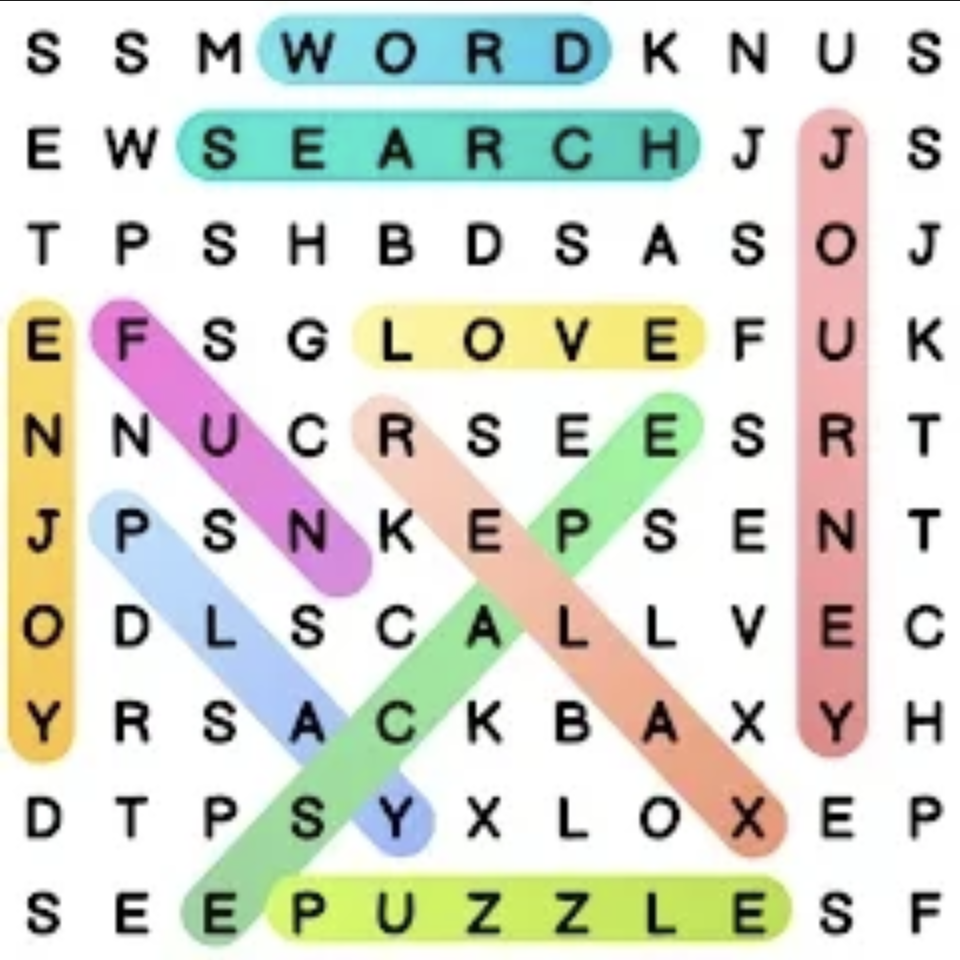
\includegraphics[width=0.4\linewidth]{tables/dataset/img_q18.png}
    \label{fig:placeholder}
\end{figure}

\textbf{Solution}: The words marked in colors are: WORD, SEARCH, JOURNEY, LOVE, RELAX, ESCAPE, FUN, PLAY, PUZZLE, ENJOY. Any answer that does not contain one of these words, or contains an extra word not in this list, is considered wrong.\\

\textbf{Question type}: \texttt{multi-to-text}\\

\textbf{Task Type}: \toggle{object-centric} \\

\textbf{Sub-Task Type}: Attribute and pattern recognition.
\end{tcolorbox}

\begin{tcolorbox}[title={Example 2}, size=title,colback=gray!10, colframe=gray, boxrule=0.5pt,
  arc=2mm, left=2mm, right=2mm, top=1mm, bottom=1mm,,breakable ]
\noindent
\textbf{Prompt}: Given a directed weighted graph. What is the shortest path from A to B?
\begin{figure}[H]
    \centering
    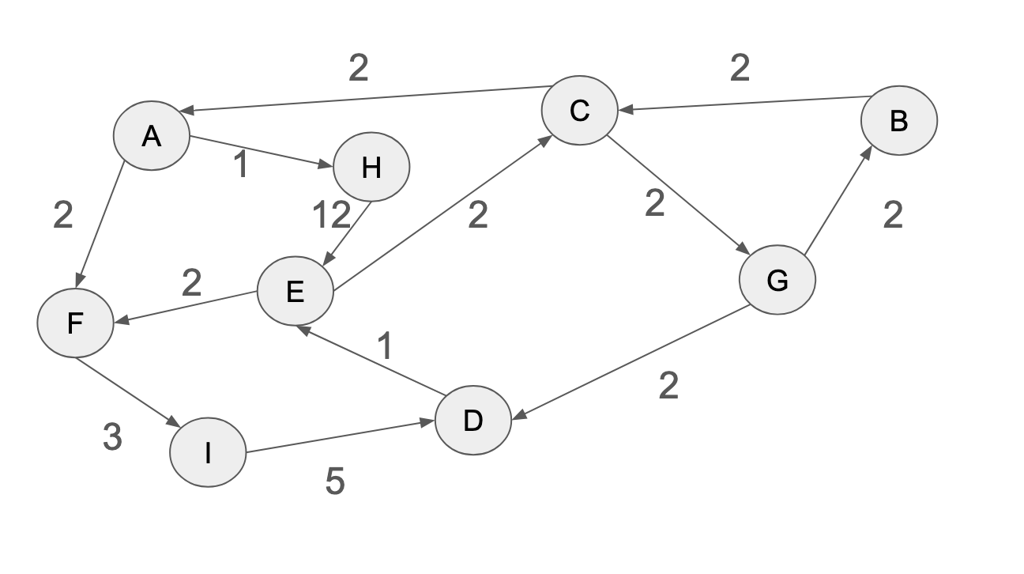
\includegraphics[width=0.5\linewidth]{tables/dataset/img_q22.png}
    \label{fig:placeholder}
\end{figure}

\textbf{Solution}: The correct answer is a shortest directed path from A to B together with its total weight. An output is correct if and only if (1) every step follows an existing directed edge in the graph (respecting arrow direction) and (2) the total weight equals the minimum over all valid directed A→B paths.

The correct shortest path is A → F → I → D → E → C → G → B with total weight 17.

This is correct because each edge in the path exists with the shown direction and weights (A→F=2, F→I=3, I→D=5, D→E=1, E→C=2, C→G=2, G→B=2), summing to 17, and no other valid directed path from A to B has a smaller total weight.

A common incorrect behavior is ignoring edge directions (treating C→A as A→C or B→C as C→B) or inventing non-existent edges (e.g., claiming C→D or D→B), producing paths that are not actually reachable in the directed graph.\\

\textbf{Question type}: \texttt{multi-to-text}\\

\textbf{Task Type}: \toggle{Abstract reasoning} \\

\textbf{Sub-Task Type}: Geometric and graph reasoning.
\end{tcolorbox}

% \begin{tcolorbox}[size=title,opacityfill=0.1,breakable]
% \noindent
% \textbf{Prompt}: Don't use any external tools. Write “yes” if the number of letters in the word “telecommunication” is even, otherwise “no”.\\
% \textbf{Solution}: The correct answer is “no”. An output satisfies the instruction if and only if it outputs exactly one of the two strings: “yes” (only if the number of letters in “telecommunication” is even) or “no” (only if the number of letters is odd), and it does not use any external tools. The word “telecommunication” contains 17 letters, which is odd, so the correct output is “no”. 

% Any output of “yes” is incorrect because it corresponds to an even letter count. A common incorrect behavior is miscounting the letters (e.g., counting 16 or 18 instead of 17) and therefore producing the wrong parity decision (“yes” instead of “no”). \\
% \textbf{Question type}: Text only\\
% \textbf{Task Type}: Language and Knowledge \\
% \textbf{Sub-Task Type}: Character-Level manipulation
% \end{tcolorbox}